\documentclass[12pt,aspectratio=169]{beamer}

% Input
\usepackage[utf8]{inputenc}
\usepackage[T1]{fontenc}
\usepackage[letterspace=100]{microtype}
\usepackage{upquote}

% Beamer
\usetheme{metropolis}
\usepackage[sfdefault]{FiraSans}
\usepackage{xcolor}
\definecolor{blue}{HTML}{002957}
\definecolor{red}{HTML}{F1563F}
\setbeamercolor{palette primary}{fg=white,bg=blue}
\setbeamercolor{title separator}{fg=red,bg=blue}
\setbeamercolor{frametitle}{fg=white,bg=blue}
\setbeamercolor{progress bar}{fg=red,bg=blue}
\setbeamercolor{alerted text}{fg=red,bg=blue}
\makeatletter
\setlength{\metropolis@titleseparator@linewidth}{2pt}
\setlength{\metropolis@progressonsectionpage@linewidth}{2pt}
\setlength{\metropolis@progressinheadfoot@linewidth}{2pt}
\makeatother

% Graphics
\usepackage{graphicx}
\usepackage{epstopdf}
\DeclareGraphicsExtensions{.png,.pdf,.eps}
\tikzset{
  invisible/.style={opacity=0},
  visible on/.style={alt={#1{}{invisible}}},
  alt/.code args={<#1>#2#3}{%
    \alt<#1>{\pgfkeysalso{#2}}{\pgfkeysalso{#3}} % \pgfkeysalso doesn't change the path
  },
}
\usetikzlibrary{arrows, shapes}

% Various
\usepackage{hyperref}
\usepackage{minted}
\usepackage{fontawesome}

% Title
\title{How Plone Excels in GatsbyJS Content Mesh}
\subtitle{Plone Conference 2019}
\date{23.10.2019}
\author{Asko Soukka}
\institute{\vspace{-0.5cm}
\includegraphics[height=1.5cm]{images/jyu-vaaka-kaksikielinen.eps}\hfill
\includegraphics[width=0.20\paperwidth]{images/plone-icon.pdf}\raisebox{0.075\paperwidth}{\fontsize{40}{40}\selectfont~+~}
\includegraphics[width=0.20\paperwidth]{images/Gatsby_Monogram.eps}}

\newcommand{\setmytemplate}{\usebackgroundtemplate{\begin{picture}(0,0)(-5,250)\footnotesize\href{https://twitter.com/datakurre}{\faTwitter~datakurre}\end{picture}\begin{picture}(0,0)(-330,298)
\includegraphics[width=0.40\paperwidth]{images/plone-icon.pdf}\end{picture}}}

\begin{document}

% define tikz styles
\definecolor{gatsby}{HTML}{663399}
\tikzstyle{block} = [rectangle, fill=gatsby, text=white,
    text width=5em, text centered, rounded corners, minimum height=4em]
\tikzstyle{example} = [rectangle, draw, dashed,
    text width=5em, text centered, rounded corners, minimum height=4em]
\tikzstyle{line} = [draw, -latex']

\setbeamertemplate{background canvas}[default]
\maketitle

%---------------------------------------------------------------------------------------

\setmytemplate
\begin{frame}{Asko Soukka}
  \textbf{Background}
  \begin{itemize}
    \item Python developer since 2002
    \item Plone developer since 2004
    \item Full-time professional since 2008
    \item GSOC mentor since 2013
    \item GatsbyJS user since 2018
  \end{itemize}
\end{frame}

%---------------------------------------------------------------------------------------

\setbeamertemplate{background canvas}[default]
\begin{frame}{University of Jyväskylä, Central Finland}
\begin{picture}(0,0)(100,141)
\includegraphics[width=1.2\paperwidth]{images/jyu-campus.jpg}
\end{picture}
\end{frame}

%---------------------------------------------------------------------------------------

\setbeamertemplate{background canvas}[default]
\section{Demo}

%---------------------------------------------------------------------------------------

\setbeamertemplate{background canvas}[default]
\section{GatsbyJS}

%---------------------------------------------------------------------------------------

\setmytemplate
\begin{frame}{Open Source}
  \textbf{GatsbyJS – the framework}
  \begin{itemize}
    \item React based website and app generator
    \item GraphQL based CMS agnostic mashup framework
    \item Server-side rendered static deployment
    \item MIT-licensed open source plugin ecosystem
  \end{itemize}
\end{frame}

%---------------------------------------------------------------------------------------

\setmytemplate
\begin{frame}{Business}
  \textbf{GatsbyJS – the company}
  \begin{itemize}
    \item Open source hobby turned into VC backed startup
    \item Copyrights owner, maintainer and evangelist
    \item Free tooling, documentation and webinars
    \item Paid cloud services with premium features
  \end{itemize}
\end{frame}

%---------------------------------------------------------------------------------------

\setmytemplate
\begin{frame}{Advantages}
  \textbf{Good}
  \begin{itemize}
    \item ''Blazingly-fast websites''
    \item Beginner friendly documentation
    \item Seamless developer experience
    \item Commitment on accessibility
    \item React ecosystem compatible
  \end{itemize}
\end{frame}

%---------------------------------------------------------------------------------------

\setmytemplate
\begin{frame}{Shortcomings}
  \textbf{Bad}
  \begin{itemize}
    \item No incremental builds
    \item Varying plugin quality
    \item GatbyJS GitHub monorepo
  \end{itemize}
  \textbf{Ugly}
  \begin{itemize}
    \item ''Overly-complicated framework and pipeline''
    \item ''Vendor lock-in for \emph{just} updating static HTML''
  \end{itemize}
\end{frame}

%---------------------------------------------------------------------------------------

\tikzstyle{decision} = [diamond, draw, aspect=2,
    text width=4.5em, text badly centered, node distance=3cm, inner sep=0pt]

\setmytemplate
\begin{frame}{Not for Everyone}
  \begin{tikzpicture}[auto]
  \small

  \node [text badly centered, text width=1.8cm]
        (d1) {React is okay};
  \node [text badly centered, below of=d1, node distance=2.5cm]
        (d1no) {\huge\raisebox{-1.35pt}{
\includegraphics[height=0.6\baselineskip]{images/Gatsby_Monogram.eps}}\hspace{-0.84em}\color{red}{\faBan}};

  \node [text badly centered, right of=d1, text width=2cm, node distance=3.5cm]
        (d2) {Content is public};
  \node [text badly centered, below of=d2, node distance=2.5cm]
        (d2no) {\huge\raisebox{-1.35pt}{
\includegraphics[height=0.6\baselineskip]{images/Gatsby_Monogram.eps}}\hspace{-0.84em}\color{red}{\faBan}};

  \node [text badly centered, text width=2.5cm, right of=d2, node distance=3.8cm]
        (d3) {Use case is read-only};
  \node [text badly centered, below of=d3, node distance=2.5cm]
        (d3no) {\huge\raisebox{-1.35pt}{
\includegraphics[height=0.6\baselineskip]{images/Gatsby_Monogram.eps}}\hspace{-0.84em}\color{red}{\faBan}};

  \node [text badly centered, right of=d3, node distance=3.2cm]
        (d3yes) {\huge\raisebox{-1.35pt}{~
\includegraphics[height=0.6\baselineskip]{images/Gatsby_Monogram.eps}}};

  \draw [->] (d1) -- (d2) node[midway] {\color{green}{\faCheck}};
  \draw [->] (d2) -- (d3) node[midway] {\color{green}{\faCheck}};
  \draw [->] (d2) -- (d3) node[midway] {\color{green}{\faCheck}};
  \draw [->] (d3) -- (d3yes) node[midway] {\color{green}{\faCheck}};

  \draw [->] (d1) -- (d1no) node[midway, left] {\color{red}{\faTimes}};
  \draw [->] (d2) -- (d2no) node[midway, left] {\color{red}{\faTimes}};
  \draw [->] (d3) -- (d3no) node[midway, left] {\color{red}{\faTimes}};

  \end{tikzpicture}
\end{frame}

%---------------------------------------------------------------------------------------

\setbeamertemplate{background canvas}[default]
\section{Content Mesh}

%---------------------------------------------------------------------------------------

\setbeamertemplate{background canvas}[default]
\begin{frame}{CMS in Disruption}
\vspace{1.01cm}
\begin{figure}
\centering
\hspace{-0.85em}
\begin{tikzpicture}
\def \n {20}
\def \N {8}
\def \radius {3cm}
\def \rd {1mm}
\def \rer {4mm}
\def \margin {8} % margin in angles, depends on the radius
\node[draw, circle] at (360:0mm) (ustar) {
\includegraphics[width=1cm]{images/plone-icon.pdf}};
\foreach \i [count=\ni from 0] in {t,1,2,3,4,5,6,7,8,9}{
  \node[draw, circle] at ({108-\ni*18}:\radius) (u\ni) {};
  \node at ({115-\ni*18}:\radius/2) {};
  \draw (ustar)--(u\ni);
}
\foreach \i in {1,3,...,11}{
  \node[circle] at ({-\i*18}:\radius) (aux) {\phantom{}};
  \draw[dotted, shorten >=3mm, shorten <=3mm] (ustar)--(aux);
}
\draw[dotted,red] (18:\radius/2) arc[start angle=18, end angle=-226, radius=\radius/2];
\end{tikzpicture}
\end{figure}
\end{frame}

%---------------------------------------------------------------------------------------

\setbeamertemplate{background canvas}[default]
\begin{frame}{CMS in Disruption}
\vspace{0.75cm}
\begin{figure}
\centering
\begin{tikzpicture}
\def \n {20}
\def \N {8}
\def \radius {3cm}
\def \rd {1mm}
\def \rer {4mm}
\def \margin {8} % margin in angles, depends on the radius
\node[draw, circle] at (360:0mm) (ustar) {
\includegraphics[width=1cm]{images/plone-icon.pdf}};
\foreach \i [count=\ni from 0] in {t,1,2,3,4,5,6,7,8,9}{
  \node[draw, circle] at ({108-\ni*18}:\radius) (u\ni) {\ifthenelse{\equal{\i}{2}}{CMS}{}\ifthenelse{\equal{\i}{5}}{\only<1>{CMS}\only<2>{
\includegraphics[width=0.5cm]{images/plone-icon.pdf}}}{}\ifthenelse{\equal{\i}{8}}{CMS}{}};
  \node at ({115-\ni*18}:\radius/2) {};
  \draw (ustar)--(u\ni);
}
\foreach \i in {1,3,...,11}{
  \node[circle] at ({-\i*18}:\radius) (aux) {\phantom{}};
  \draw[dotted, shorten >=3mm, shorten <=3mm] (ustar)--(aux);
}
\draw[dotted,red] (18:\radius/2) arc[start angle=18, end angle=-226, radius=\radius/2];
\end{tikzpicture}
\end{figure}
\end{frame}

%---------------------------------------------------------------------------------------

\setbeamertemplate{background canvas}[default]
\begin{frame}{CMS in Disruption}
\vspace{0.75cm}
\begin{figure}
\centering
\begin{tikzpicture}
\def \n {20}
\def \N {8}
\def \radius {3cm}
\def \rd {1mm}
\def \rer {4mm}
\def \margin {8} % margin in angles, depends on the radius
\node[draw, circle] at (360:0mm) (ustar) {
\includegraphics[width=1cm]{images/Gatsby_Monogram.eps}};
\foreach \i [count=\ni from 0] in {t,1,2,3,4,5,6,7,8,9}{
  \node[draw, circle] at ({108-\ni*18}:\radius) (u\ni) {\ifthenelse{\equal{\i}{2}}{CMS}{}\ifthenelse{\equal{\i}{5}}{
\includegraphics[width=0.5cm]{images/plone-icon.pdf}}{}\ifthenelse{\equal{\i}{8}}{
\includegraphics[width=0.5cm]{images/plone-icon.pdf}}{}};
  \node at ({115-\ni*18}:\radius/2) {};
  \draw (ustar)--(u\ni);
}
\foreach \i in {1,3,...,11}{
  \node[circle] at ({-\i*18}:\radius) (aux) {\phantom{}};
  \draw[dotted, shorten >=3mm, shorten <=3mm] (ustar)--(aux);
}
\draw[dotted,red] (18:\radius/2) arc[start angle=18, end angle=-226, radius=\radius/2];
\end{tikzpicture}
\end{figure}
\end{frame}

%---------------------------------------------------------------------------------------

\setbeamertemplate{background canvas}[default]
\begin{frame}{Content Mesh / JAMstack}
\vspace{0.75cm}
\begin{figure}
\centering
\begin{tikzpicture}
\def \n {20}
\def \N {8}
\def \radius {3cm}
\def \rd {1mm}
\def \rer {4mm}
\def \margin {8} % margin in angles, depends on the radius
\node[draw, circle] at (360:0mm) (ustar) {
\includegraphics[width=1cm]{images/Gatsby_Monogram.eps}};
\foreach \i [count=\ni from 0] in {t,1,2,3,4,5,6,7,8,9}{
  \node[draw, circle] at ({108-\ni*18}:\radius) (u\ni) {\ifthenelse{\equal{\i}{2}}{CMS}{}\ifthenelse{\equal{\i}{5}}{
\includegraphics[width=0.5cm]{images/plone-icon.pdf}}{}\ifthenelse{\equal{\i}{8}}{
\includegraphics[width=0.5cm]{images/plone-icon.pdf}}{}};
  \node at ({115-\ni*18}:\radius/2) {};
  \draw (ustar)--(u\ni);
}
\begin{scope}[every node/.style={shift={(7cm,1.5cm)},scale=0.8}]
\node[draw, circle] at (360:0mm) (ustar2) {
\includegraphics[width=0.8cm]{images/Gatsby_Monogram.eps}};
\foreach \i [count=\ni from 0] in {t,6,7,8}{
  \node[draw, circle] at ({40-\ni*28}:{\radius*0.7}) (u2\ni) {\ifthenelse{\equal{\i}{5}}{CMS}{}\ifthenelse{\equal{\i}{8}}{CMS}{}};
  \draw (ustar2)--(u2\ni);
}
\draw (u\ni)--(ustar2);
\draw (u5)--(ustar2);
\end{scope}
\begin{scope}[every node/.style={shift={(7cm,-1.5cm)},scale=0.8}]
\node[draw, circle] at (360:0mm) (ustar3) {
\includegraphics[width=0.8cm]{images/Gatsby_Monogram.eps}};
\foreach \i [count=\ni from 0] in {t,7,8,9}{
  {\ifthenelse{\equal{\i}{7}}{}{
    \node[draw, circle] at ({208-\ni*28}:{\radius*0.7}) (u3\ni) {\ifthenelse{\equal{\i}{5}}{CMS}{}\ifthenelse{\equal{\i}{8}}{CMS}{}};
  \draw (ustar3)--(u3\ni);
  }};
}
\draw (u2\ni)--(ustar3);
\draw (u8)--(ustar3);
\end{scope}
\end{tikzpicture}
\end{figure}
\end{frame}

%---------------------------------------------------------------------------------------

\setbeamertemplate{background canvas}[default]
\section{Ecosystem}

%---------------------------------------------------------------------------------------

\setmytemplate
\begin{frame}{Plugin Categories}
  \begin{tikzpicture}[node distance=3.5cm, auto]
  \node [block] (source) {\textbf{SOURCE}};
  \node [block, right of=source, text width=3.5cm, node distance=3.9cm, visible on=<3->] (transformer) {\textbf{TRANSFORMER}};
  \node [block, right of=transformer, node distance=3.9cm, visible on=<5->] (theme) {\textbf{THEME}};
  \node [example, below of=source, node distance=2.5cm, visible on=<2->] (source_example) {images};
  \node [example, below of=transformer, text width=3.5cm, node distance=2.5cm, visible on=<4->] (transformer_example) {scales};
  \node [example, below of=theme, node distance=2.5cm, visible on=<6->] (theme_example) {gallery};
  \end{tikzpicture}
\end{frame}

%---------------------------------------------------------------------------------------

\setbeamertemplate{background canvas}[default]
\begin{frame}[standout]
\centering
\Huge All {\color{red}{plugins}} are equal
\par
\normalsize
categories are not enforced
\end{frame}

%---------------------------------------------------------------------------------------

\setbeamertemplate{background canvas}[default]
\section{Themes}

%---------------------------------------------------------------------------------------

\setmytemplate
\begin{frame}{Gatsby Themes}
  \textbf{Experiment on maintainable boilerplate}
  \begin{itemize}
    \item Packages with pre-configured components
    \item Configuration possible with plugin options
    \item Overridable or extendable by shadowing
  \end{itemize}
  \vspace{0.5cm}
  \begin{tikzpicture}[node distance=3cm, auto]
  \node [block, visible on=<2->] (jboa) {\textbf{JBOA}};
  \node [block, right of=jboa, visible on=<3->] (custom) {\textbf{???}};
  \node [block, right of=custom, visible on=<4->] (profit) {\textbf{PROFIT}};
  \end{tikzpicture}
\end{frame}

%---------------------------------------------------------------------------------------

\setmytemplate
\begin{frame}{Example ''theme'' \texttt{gatsby-theme-coverflow}}
\frame{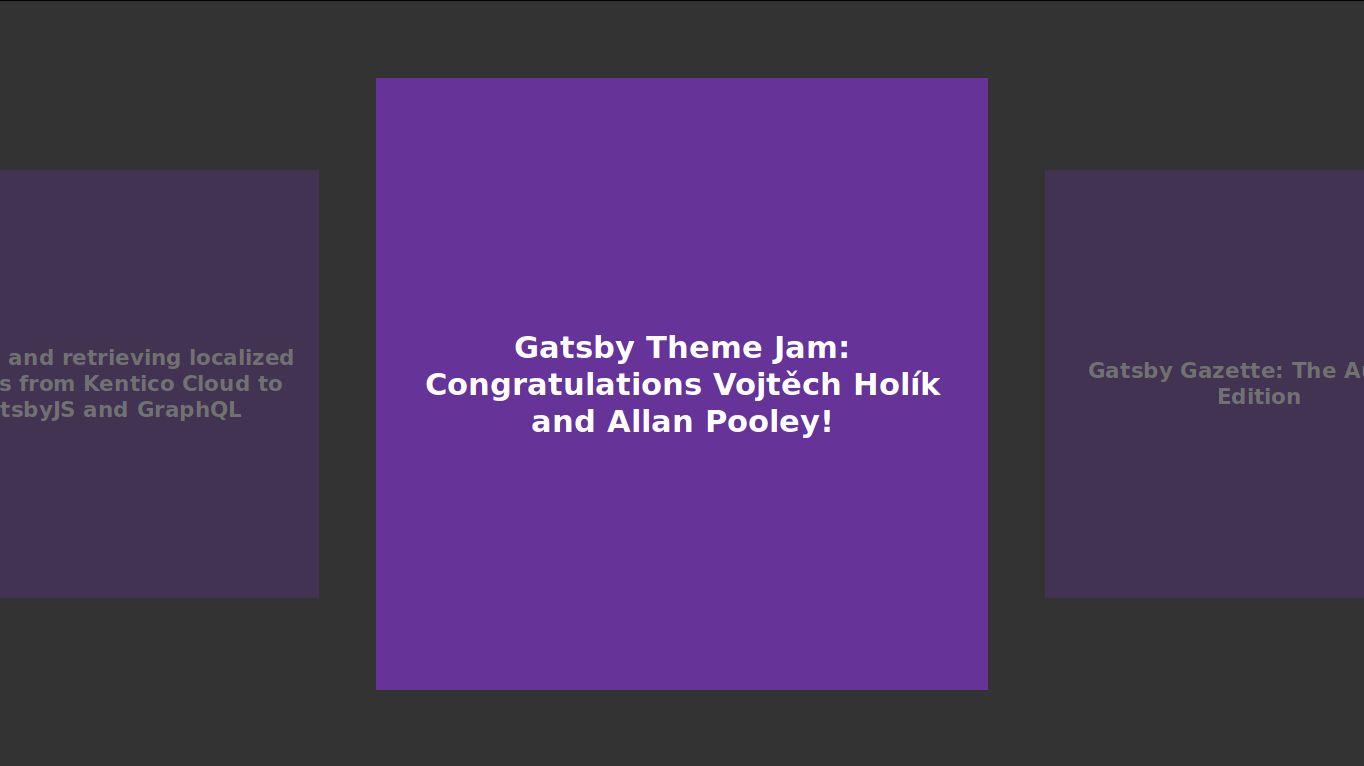
\includegraphics[height=0.6\paperheight]{images/gatsby-theme-coverflow.png}}
\href{https://datakurre.github.io/gatsby-theme-coverflow/\#1}{datakurre.github.io/gatsby-theme-coverflow}
\end{frame}

%---------------------------------------------------------------------------------------

\setmytemplate
\begin{frame}[fragile]{Example ''theme'' configuration}
\footnotesize
\begin{minted}{javascript}
{
  resolve: "gatsby-theme-coverflow",
  options: {
    path: "gatsby-blog",
    query: `{ allCoverPages: allFeedGatsbyBlog {
              edges {
                node {
                  title
                  link
                }
              }
            } }`
  }
}
\end{minted}
\end{frame}

%---------------------------------------------------------------------------------------

\setbeamertemplate{background canvas}[default]
\section{Plone}

%---------------------------------------------------------------------------------------

\setmytemplate
\begin{frame}{Out of the Box}
  \textbf{Enablers}
  \begin{itemize}
    \item Hierarcical content management
    \item Flexible publication workflows
    \item Customizable content types
    \item Effective and expiration dates
    \item High quality extensible REST API
  \end{itemize}
\end{frame}


%---------------------------------------------------------------------------------------

\setmytemplate
\begin{frame}{Excellences}
  \textbf{Curated use-cases}
  \begin{itemize}
    \item Standalone spin-off web sites
    \item CMS part of GatsbyJS web apps
    \item Content configuration management
    \item[]<2>\vspace{\baselineskip}\hspace{-1.9em}\textbf{Seen challenges}\par
    \item<2> WYSIWYG $\,\to\,$ WYSIWYM
    \item<2> Release management
  \end{itemize}
\end{frame}

%---------------------------------------------------------------------------------------

\setmytemplate
\begin{frame}{Status of \texttt{gatsby-source-plone}}
  \textbf{Done}
  \begin{itemize}
    \item Incremental Plone content sourcing
    \item Selectable site root with \texttt{baseURL} option
    \item Support for rich text, images and files
    \item Rich text to React w/ Gatsby links and images
    \item GraphQL queries by \texttt{\_path} or by hierarchy
    \item Websocket-ready for instant \texttt{develop} updates
  \end{itemize}
\end{frame}

%---------------------------------------------------------------------------------------

\setmytemplate
\begin{frame}{Future of \texttt{gatsby-source-plone}}
  \textbf{To do}
  \begin{itemize}
    \item Support custom rich text, image and file fields
    \vspace{0.5\baselineskip}\par
    \emph{Issue:}~Only fields \texttt{text}, \texttt{image} and \texttt{file} are supported
    \vspace{0.5\baselineskip}\par
    \item Path prefixing or namespacing support\\ for multiple plugin instances
    \vspace{0.5\baselineskip}\par
    \emph{Issue:}~Instances may override each others' nodes
    \vspace{0.5\baselineskip}\par
  \end{itemize}
\end{frame}

%---------------------------------------------------------------------------------------

\setbeamertemplate{background canvas}[default]
\section{Get Started}

%---------------------------------------------------------------------------------------

\setmytemplate
\begin{frame}[fragile]{Get Started with \texttt{gatsby-source-plone}\hfill1/3}
\vspace{0.8\baselineskip}
\textbf{Create a new project}
\footnotesize
\begin{minted}{sh}
$ npx gatsby new my-gatsby-project
$ cd my-gatsby-project
$ yarn add git+https://github.com/collective/gatsby-source-plone
\end{minted}
\normalsize
\textbf{Add a Plone source in} \texttt{./gatsby-config.js} \textbf{with}
\footnotesize
\begin{minted}{javascript}
plugins: [
  { resolve: 'gatsby-source-plone',
    options: {
      baseUrl: 'https://plonedemo.kitconcept.com/en',
    },
  },
\end{minted}
\end{frame}

%---------------------------------------------------------------------------------------

\setmytemplate
\begin{frame}[fragile,t]{Get Started with \texttt{gatsby-source-plone}\hfill2/3}
\textbf{Start GatsbyJS development server}
\footnotesize
\begin{minted}{sh}
$ yarn gatsby develop
\end{minted}
\normalsize
\textbf{Open browser at}~~\texttt{\href{http://localhost:8000/___graphql}{http://localhost:8000/\_\_\_graphql}}
\begin{picture}(280,238)(28,0)
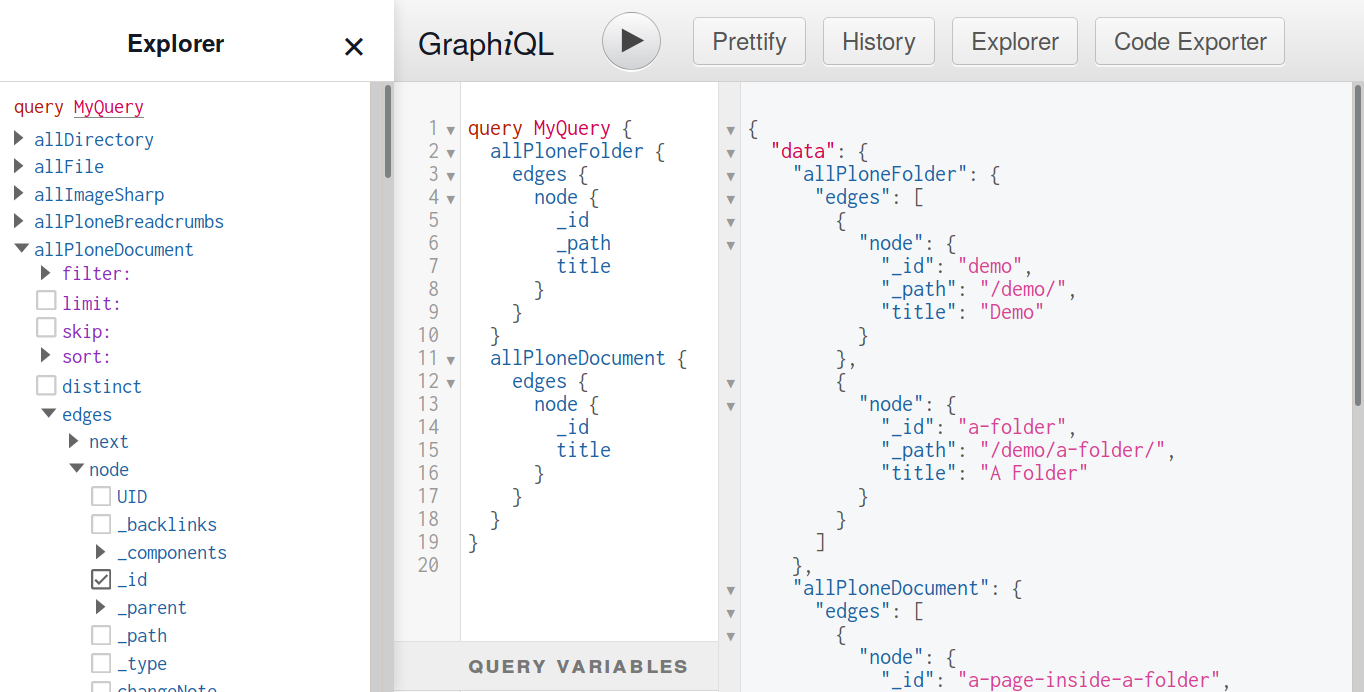
\includegraphics[width=\paperwidth]{images/graphiql.png}
\end{picture}
\end{frame}

%---------------------------------------------------------------------------------------

\setmytemplate
\begin{frame}{Get Started with \texttt{gatsby-source-plone}\hfill3/3}
  \textbf{Learn GatsbyJS}
  \begin{itemize}
    \item \href{https://www.gatsbyjs.org/tutorial/}{gatsbyjs.org/tutorial}
    \item \href{https://collective.github.io/gatsby-source-plone/tutorial/}{collective.github.io/gatsby-source-plone}
  \end{itemize}
  \textbf{Ask for help}
  \begin{itemize}
    \item \href{https://github.com/collective/gatsby-source-plone/issues}{github.com/collective/gatsby-source-plone/issues}
  \end{itemize}
\end{frame}

%---------------------------------------------------------------------------------------

\setmytemplate
\begin{frame}{More of \texttt{gatsby-source-plone}}
  \textbf{Web site examples}
  \begin{itemize}
    \item \href{https://github.com/collective/gatsby-source-plone/tree/master/demo}{github.com/collective/gatsby-source-plone}
    \item \href{https://github.com/collective/gatsby-starter-plone}{github.com/collective/gatsby-starter-plone}
  \end{itemize}
  \textbf{Landing page example}
  \begin{itemize}
    \item \href{https://github.com/datakurre/gatsby-starter-plone-brochure}{github.com/datakurre/gatsby-starter-plone-brochure}
  \end{itemize}
  \textbf{Content configuration example}
  \begin{itemize}
    \item \href{https://github.com/datakurre/gatsby-theme-ds-player}{github.com/datakurre/gatsby-theme-ds-player}
  \end{itemize}
\end{frame}

%---------------------------------------------------------------------------------------

\setbeamertemplate{background canvas}[default]
\begin{frame}[standout]
\vfill

\includegraphics[height=0.50\paperheight]{images/plone-icon-hearts.png}
\par
\href{https://datakurre.github.io/ploneconf2019/}{datakurre.github.io/ploneconf2019}
\end{frame}

%---------------------------------------------------------------------------------------

\end{document}
